\chapter{面向雨天的车道线检测算法设计}
\label{chap:algorithm_design}

\section{引言}
\label{sec:intro_4}

车道线检测作为高级驾驶辅助系统的核心感知任务之一，其检测精度直接影响车道保持、路径规划等后续模块的可靠性。在晴朗天气条件下，基于深度学习的方法如SCNN\cite{pan2018spatial}、基于实例分割的端到端方法\cite{neven2018}和RESA\cite{zheng2021}已在多个公开数据集上取得了优异的检测性能。然而，当车辆行驶于雨天环境时，雨滴附着于镜头表面形成局部遮挡，路面积水产生的镜面反射破坏车道线的连续性与对比度，同时雨纹噪声导致图像整体信噪比显著下降。上述因素共同作用，使得现有模型在雨天场景下的漏检率与误检率急剧上升，严重制约了ADAS系统在恶劣天气下的可用性。

针对上述问题，本章以 CLRNet 作为基线模型，分析其在雨天场景下的失效机理，并据此设计面向雨天干扰的轻量化抗干扰模块。本文的改进重点不在于额外叠加复杂的图像增强分支，而是在特征层中引入“频域门控 + 方向注意力”组合模块，以较小的结构改动提升模型对雨纹噪声、局部遮挡和反射伪边缘的抑制能力。围绕这一思路，本章先对 CLRNet 的整体架构、特征提取流程及先验锚点设计进行分析，说明其在雨天条件下性能退化的原因；再从频域角度刻画雨滴、水膜反射等干扰因素对车道线特征表达的影响；随后阐述抗干扰模块的设计原则、实现方式及其与 CLRNet 的融合位置；最后给出与模块结构相匹配的训练策略说明。

\section{CLRNet模型结构分析}
\label{sec:clrnet_analysis}

CLRNet（Cross Layer Refinement Network for Lane Detection）是近年来车道线检测领域具有代表性的方法之一，其在LaneATT的基础上引入了跨层特征精炼机制，有效提升了车道线定位精度与实例区分能力。本课题选择CLRNet作为基线模型，主要基于以下两点考虑：其一，CLRNet在多个公开数据集上取得了领先性能，且模型结构具有较好的可扩展性；其二，其基于行锚点的车道线表示方式兼顾了检测效率与精度，适合后续在嵌入式平台上的部署需求。

\subsection{网络整体架构}

CLRNet的整体架构由三部分构成：主干特征提取网络、跨层特征精炼模块以及车道线预测头。主干网络通常采用ResNet或DLA等经典卷积架构，负责从输入图像中提取多尺度特征图。设输入图像尺寸为$H \times W \times 3$，经过主干网络后得到多级特征图$\{\mathbf{F}_l\}_{l=1}^L$，其中$\mathbf{F}_l \in \mathbb{R}^{C_l \times H_l \times W_l}$，$l$表示特征层级，$C_l$为通道数。

跨层特征精炼模块是CLRNet的核心创新所在。与传统的FPN结构不同，CLRNet采用了一种基于通道注意力的特征交互机制，通过高层语义信息引导低层特征的加权融合，从而增强车道线这类细长目标的特征响应。具体而言，对于第$l$级特征图$\mathbf{F}_l$，首先利用全局平均池化获得通道描述向量，随后通过全连接层生成注意力权重，对$\mathbf{F}_l$的各通道进行重标定。精炼后的特征图可表示为：
\begin{equation}
	\tilde{\mathbf{F}}_l = \mathbf{F}_l \odot \sigma(\mathbf{W}_2 \delta(\mathbf{W}_1 \text{GAP}(\mathbf{F}_l)))
\end{equation}
其中，$\text{GAP}(\cdot)$为全局平均池化，$\delta$为ReLU激活函数，$\sigma$为Sigmoid函数，$\mathbf{W}_1$和$\mathbf{W}_2$为可学习参数。

车道线预测头将车道线检测建模为行方向上的分类问题。将图像在垂直方向上划分为$H_r$个行锚点，对于每一行，预测头输出一个$W_r$维的分类向量，表示车道线在该行中的水平位置。同时，预测头还输出车道线的存在性置信度以及纵向延伸范围。这种表示方式避免了传统分割方法中复杂的后处理步骤，显著提升了推理效率。图~\ref{fig:clrnetmodel}直观展示了CLRNet\cite{zheng2022clrnet}模型的整体架构。

\begin{figure}[htbp]
	\centering
	\includegraphics[width=\textwidth]{image/chap04/框架图.png}
	\small
	\caption{CLRNet 整体结构示意图（改绘自文献\cite{zheng2022clrnet})}
	\label{fig:clrnetmodel}
\end{figure}


\subsection{雨天场景下的性能局限}

尽管CLRNet在常规天气下表现优异，但将其直接应用于雨天图像时，检测性能出现明显衰减。通过分析模型在自建雨天数据集上的失效案例，可将失效模式归纳为以下三类：

第一，雨滴遮挡导致的特征中断。当雨滴附着于镜头表面时，对应图像区域产生严重的模糊和形变，主干网络提取的局部特征中车道线边缘响应大幅减弱。由于CLRNet的跨层精炼机制依赖于连续的空间特征，当某一局部区域的特征缺失时，精炼过程无法有效恢复车道线的连续性，最终导致预测的行锚点位置出现断崖式跳变。

第二，水膜反射引发的伪边缘响应。路面水膜在光照下形成镜面反射，产生与其实车道线高度相似的亮条纹。卷积神经网络的前几层对图像梯度信息较为敏感，水膜反射产生的强边缘易被误激活为车道线候选特征。在后续的注意力精炼过程中，由于伪边缘与真实车道线在局部形态上难以区分，模型可能将较高的置信度赋予错误位置，造成误检。

第三，整体对比度下降导致的行分类模糊。雨水覆盖使得整幅图像的对比度降低，车道线与路面的灰度差异减小。CLRNet的行分类预测头依赖于特征图中对应位置的判别性信息，当特征响应整体减弱时，分类概率分布趋于平坦，峰值不显著，导致定位精度下降，甚至因置信度低于阈值而被完全漏检。

上述分析表明，提升CLRNet在雨天环境下的鲁棒性，关键在于设计一种能够在特征层面有效抑制雨纹噪声、同时增强车道线结构响应的轻量化模块，而非简单地在前端叠加图像去雨预处理。

\begin{figure}[htbp]
	\centering
	\begin{subfigure}[b]{0.48\textwidth}
		\centering
		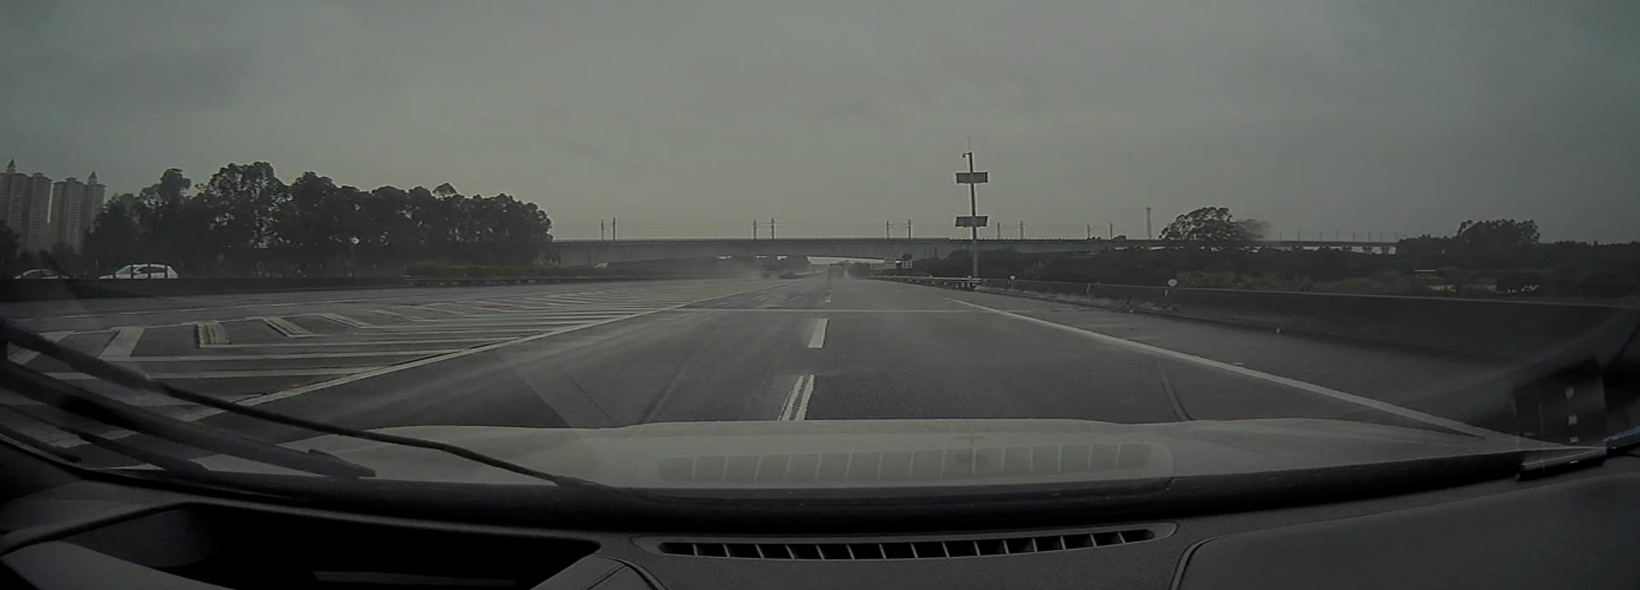
\includegraphics[width=\textwidth]{image/chap03/s4_2427000_原图.jpg}
		\caption{原始场景}
	\end{subfigure}
	\hfill
	\begin{subfigure}[b]{0.48\textwidth}
		\centering
		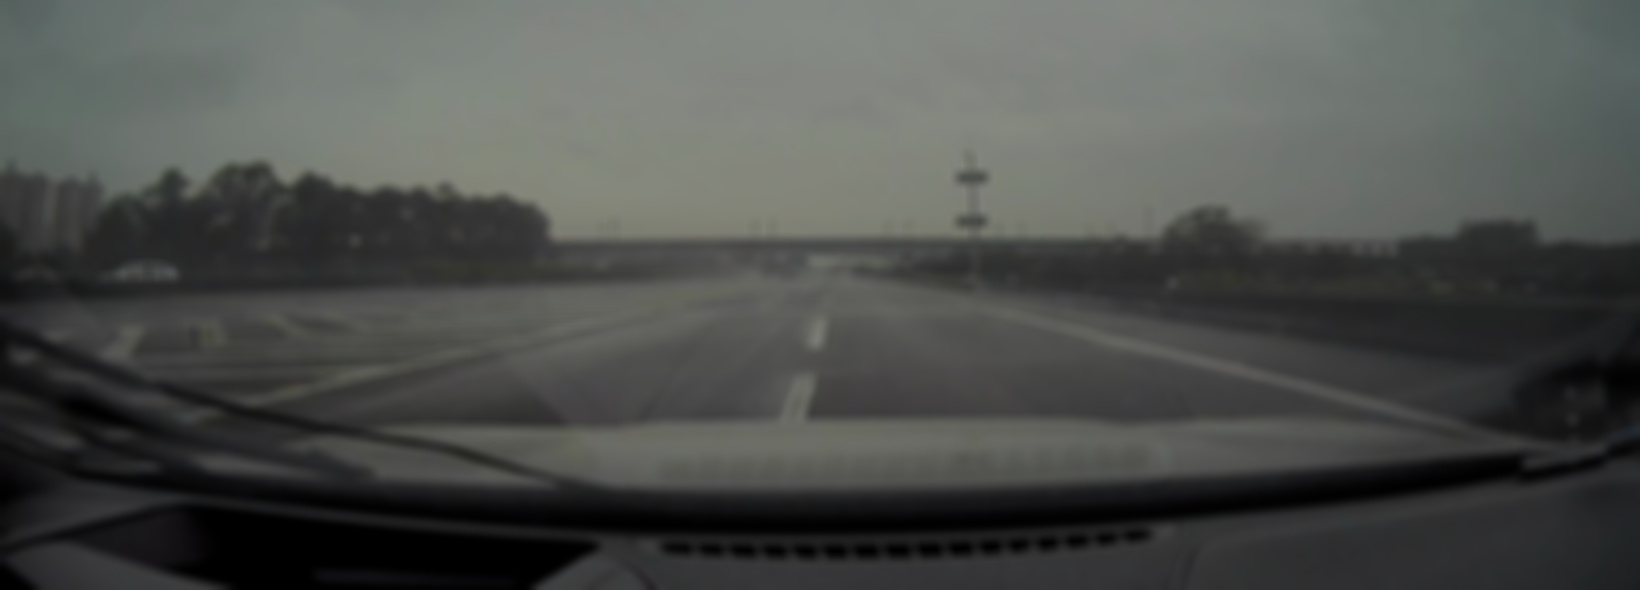
\includegraphics[width=\textwidth]{image/chap03/s4_2427000_高斯模糊.jpg}
		\caption{模糊与雨纹干扰}
	\end{subfigure}

	\vspace{0.5em}

	\begin{subfigure}[b]{0.48\textwidth}
		\centering
		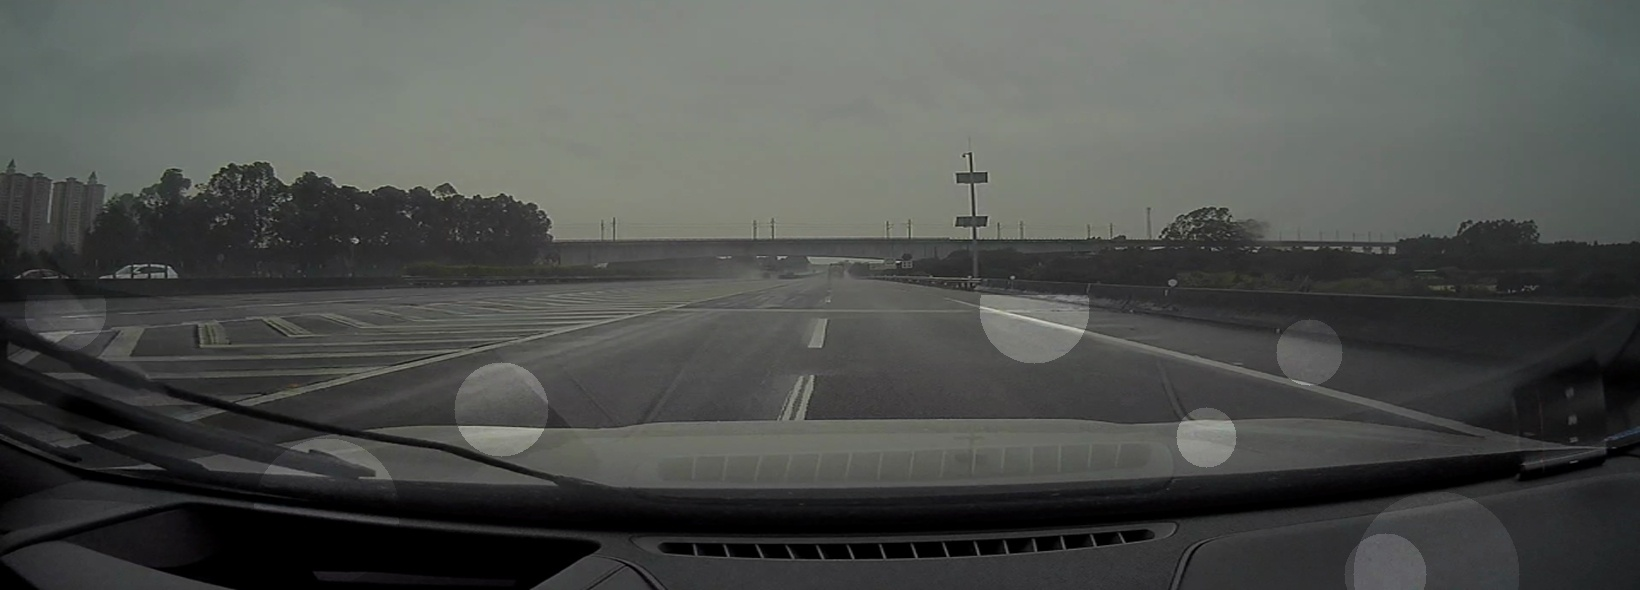
\includegraphics[width=\textwidth]{image/chap03/s4_2427000_重度水膜反射.jpg}
		\caption{水膜反射伪边缘}
	\end{subfigure}
	\hfill
	\begin{subfigure}[b]{0.48\textwidth}
		\centering
		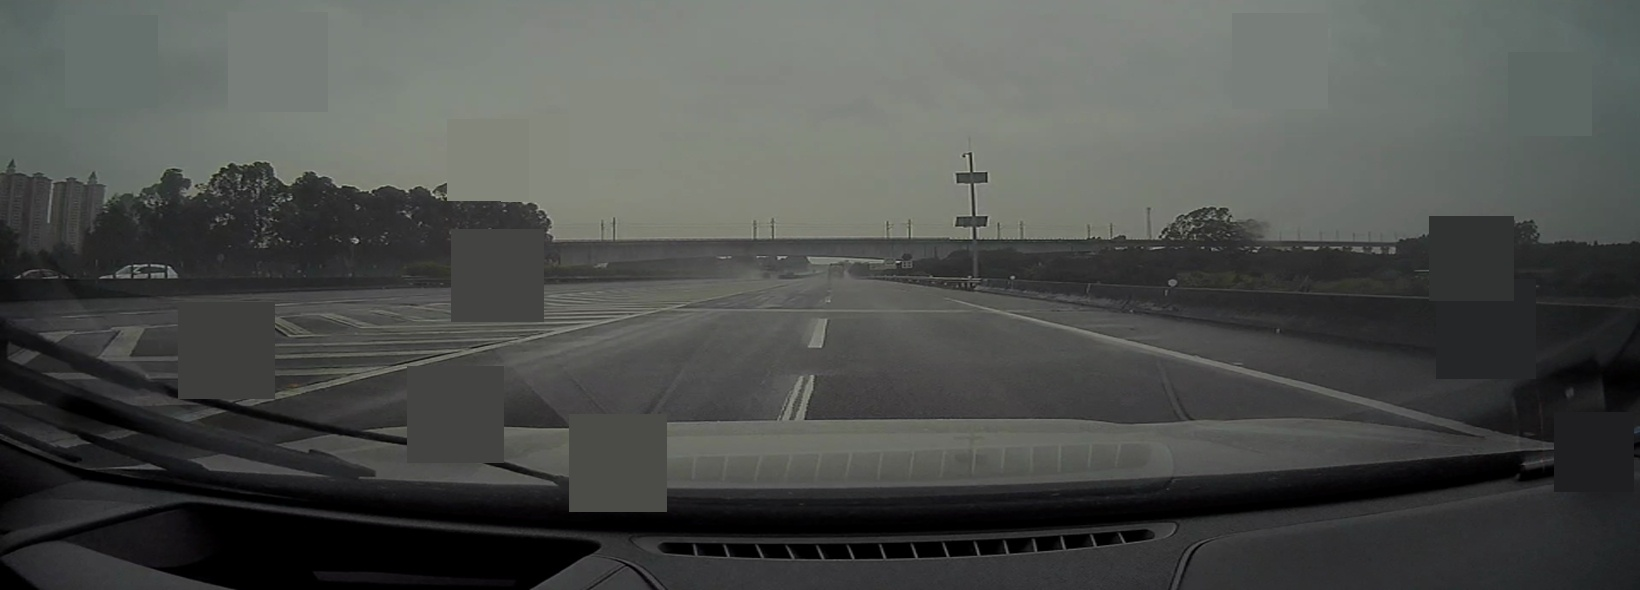
\includegraphics[width=\textwidth]{image/chap03/s4_2427000_重度遮挡.jpg}
		\caption{局部遮挡与断裂}
	\end{subfigure}
	\caption{雨天场景中典型失效诱因示例}
	\label{fig:rain_failure_modes}
\end{figure}

\section{雨天干扰分析与模块设计}
\label{sec:rain_interference}

\subsection{雨天干扰的频域特性分析}

为设计针对性的抗干扰机制，首先需要对雨天图像的干扰模式进行定量分析。雨天图像可建模为清晰背景图像与雨纹噪声层的叠加\cite{zhang2018}：
\begin{equation}
	\mathbf{I}_{\text{rain}}(x) = \mathbf{I}_{\text{clean}}(x) + \mathbf{R}(x)
\end{equation}
其中，$\mathbf{I}_{\text{clean}}$表示未受雨水干扰的理想图像，$\mathbf{R}$为雨纹层，包括动态雨滴、静态水膜反射以及附着雨滴等。

从频域角度考察雨纹噪声的分布特性。对多幅雨天车道线图像进行二维傅里叶变换并统计平均功率谱，可发现雨纹成分主要集中在高频区域，表现为方向性的能量尖峰（对应于雨滴的运动轨迹）以及弥散的高频噪声（源于水膜反射的随机纹理）。相比之下，车道线作为结构化的人造目标，其边缘信息在频域中体现为中高频段的定向能量分布，但整体能量峰值低于雨纹噪声。

这一频域差异为设计抗干扰模块提供了重要启示：若能在特征提取阶段对高频成分进行自适应门控，选择性抑制雨纹对应的噪声分量而保留车道线边缘信息，则有望在不显著增加计算开销的前提下提升特征质量。

\subsection{轻量级抗干扰模块的设计思路}

基于上述分析，本文提出一种轻量化抗干扰模块，其设计遵循以下三项原则：
\begin{enumerate}
	\item \textbf{从特征层抑制干扰而非重建图像}：直接在 backbone 输出特征上处理雨天干扰，避免独立去雨网络带来的额外计算负担及任务失配。
	\item \textbf{同时兼顾频率选择性与方向敏感性}：一方面利用频域门控压制与雨纹相关的高频噪声，另一方面利用方向注意力强化车道线这一细长目标的结构连续性。
	\item \textbf{保持实现简单与部署友好}：模块仅由 FFT 操作、深度卷积、$1\times1$ 卷积和残差连接组成，便于嵌入现有 CLRNet 框架，并兼顾工程实现的简洁性。
\end{enumerate}

结合当前模块设计，整体结构由两个并行分支构成：一是频域门控分支（Frequency Gate），通过对特征图进行二维傅里叶变换，对高频区域施加可学习衰减；二是方向注意力分支（Directional Attention），通过多组深度可分离卷积提取不同方向上的局部结构响应，并生成通道级注意力图。两个分支的输出再以残差形式与原始特征融合，从而在尽量不破坏主干特征分布的前提下完成抗干扰增强。模块的具体计算路径以及其在 CLRNet 中的插入方式，将在下一节结合结构示意图进一步说明。

\section{抗干扰机制实现与融合}
\label{sec:anti_interference}

\subsection{频域门控与方向注意力模块的具体实现}

本节详细阐述FGM模块的具体实现细节。模块的整体计算流程如下所述，其前向传播过程可由以下步骤描述。

\textbf{步骤一：频域门控分支。} 对输入特征图 $\mathbf{X} \in \mathbb{R}^{C \times H \times W}$ 做二维傅里叶变换，得到频谱表示 $\mathcal{F}(\mathbf{X})$。随后根据频率半径构造高频掩码，对高于阈值的区域施加可学习门控系数，从而抑制雨纹、反光伪边缘等高频噪声分量。若记高频掩码为 $\mathbf{M}_{\text{high}}$，每个通道的可学习门控向量为 $\mathbf{g}$，则门控后的频谱幅值可表示为
\begin{equation}
	\mathcal{A}' = \mathcal{A} \odot \left(1 - \mathbf{M}_{\text{high}} + \mathbf{M}_{\text{high}} \odot \sigma(\mathbf{g})\right)
\end{equation}
其中 $\mathcal{A}$ 为原始频谱幅值，$\sigma(\cdot)$ 为 Sigmoid 函数。经过逆傅里叶变换后得到频域增强特征，并采用小比例残差方式与输入特征相加，以避免强行滤除有用边缘信息。

\textbf{步骤二：方向注意力分支。} 为了增强车道线的方向连续性，本文在空间域中并行引入方向注意力。具体做法是对输入特征施加多组深度可分离卷积，获得多个方向响应特征图，再将这些特征在通道维度拼接后，通过 $1\times1$ 卷积和 Sigmoid 激活生成注意力图：
\begin{equation}
	\mathbf{A}_{\text{dir}} = \sigma\left(\text{Conv}_{1\times1}\left([\mathbf{D}_1(\mathbf{X}),\mathbf{D}_2(\mathbf{X}),\ldots,\mathbf{D}_B(\mathbf{X})]\right)\right)
\end{equation}
其中 $\mathbf{D}_b(\cdot)$ 表示第 $b$ 个方向卷积分支。最终将方向注意力作用于原始特征图，得到 $\mathbf{X}_{\text{dir}} = \mathbf{X} \odot \mathbf{A}_{\text{dir}}$。

\textbf{步骤三：残差融合输出。} 结合当前实现，模块最终并未引入额外的光照增强分支，而是仅保留频域门控和方向注意力两个核心分支。若记两分支输出分别为 $\mathbf{X}_{\text{freq}}$ 和 $\mathbf{X}_{\text{dir}}$，则模块输出为
\begin{equation}
	\tilde{\mathbf{X}} = \mathbf{X} + \lambda \left(\mathbf{X}_{\text{freq}} + \mathbf{X}_{\text{dir}}\right)
\end{equation}
其中 $\lambda$ 为可学习的残差缩放系数。该设计保证了模块在训练初期更接近恒等映射，有助于稳定收敛。

\begin{figure}[htbp]
	\centering
	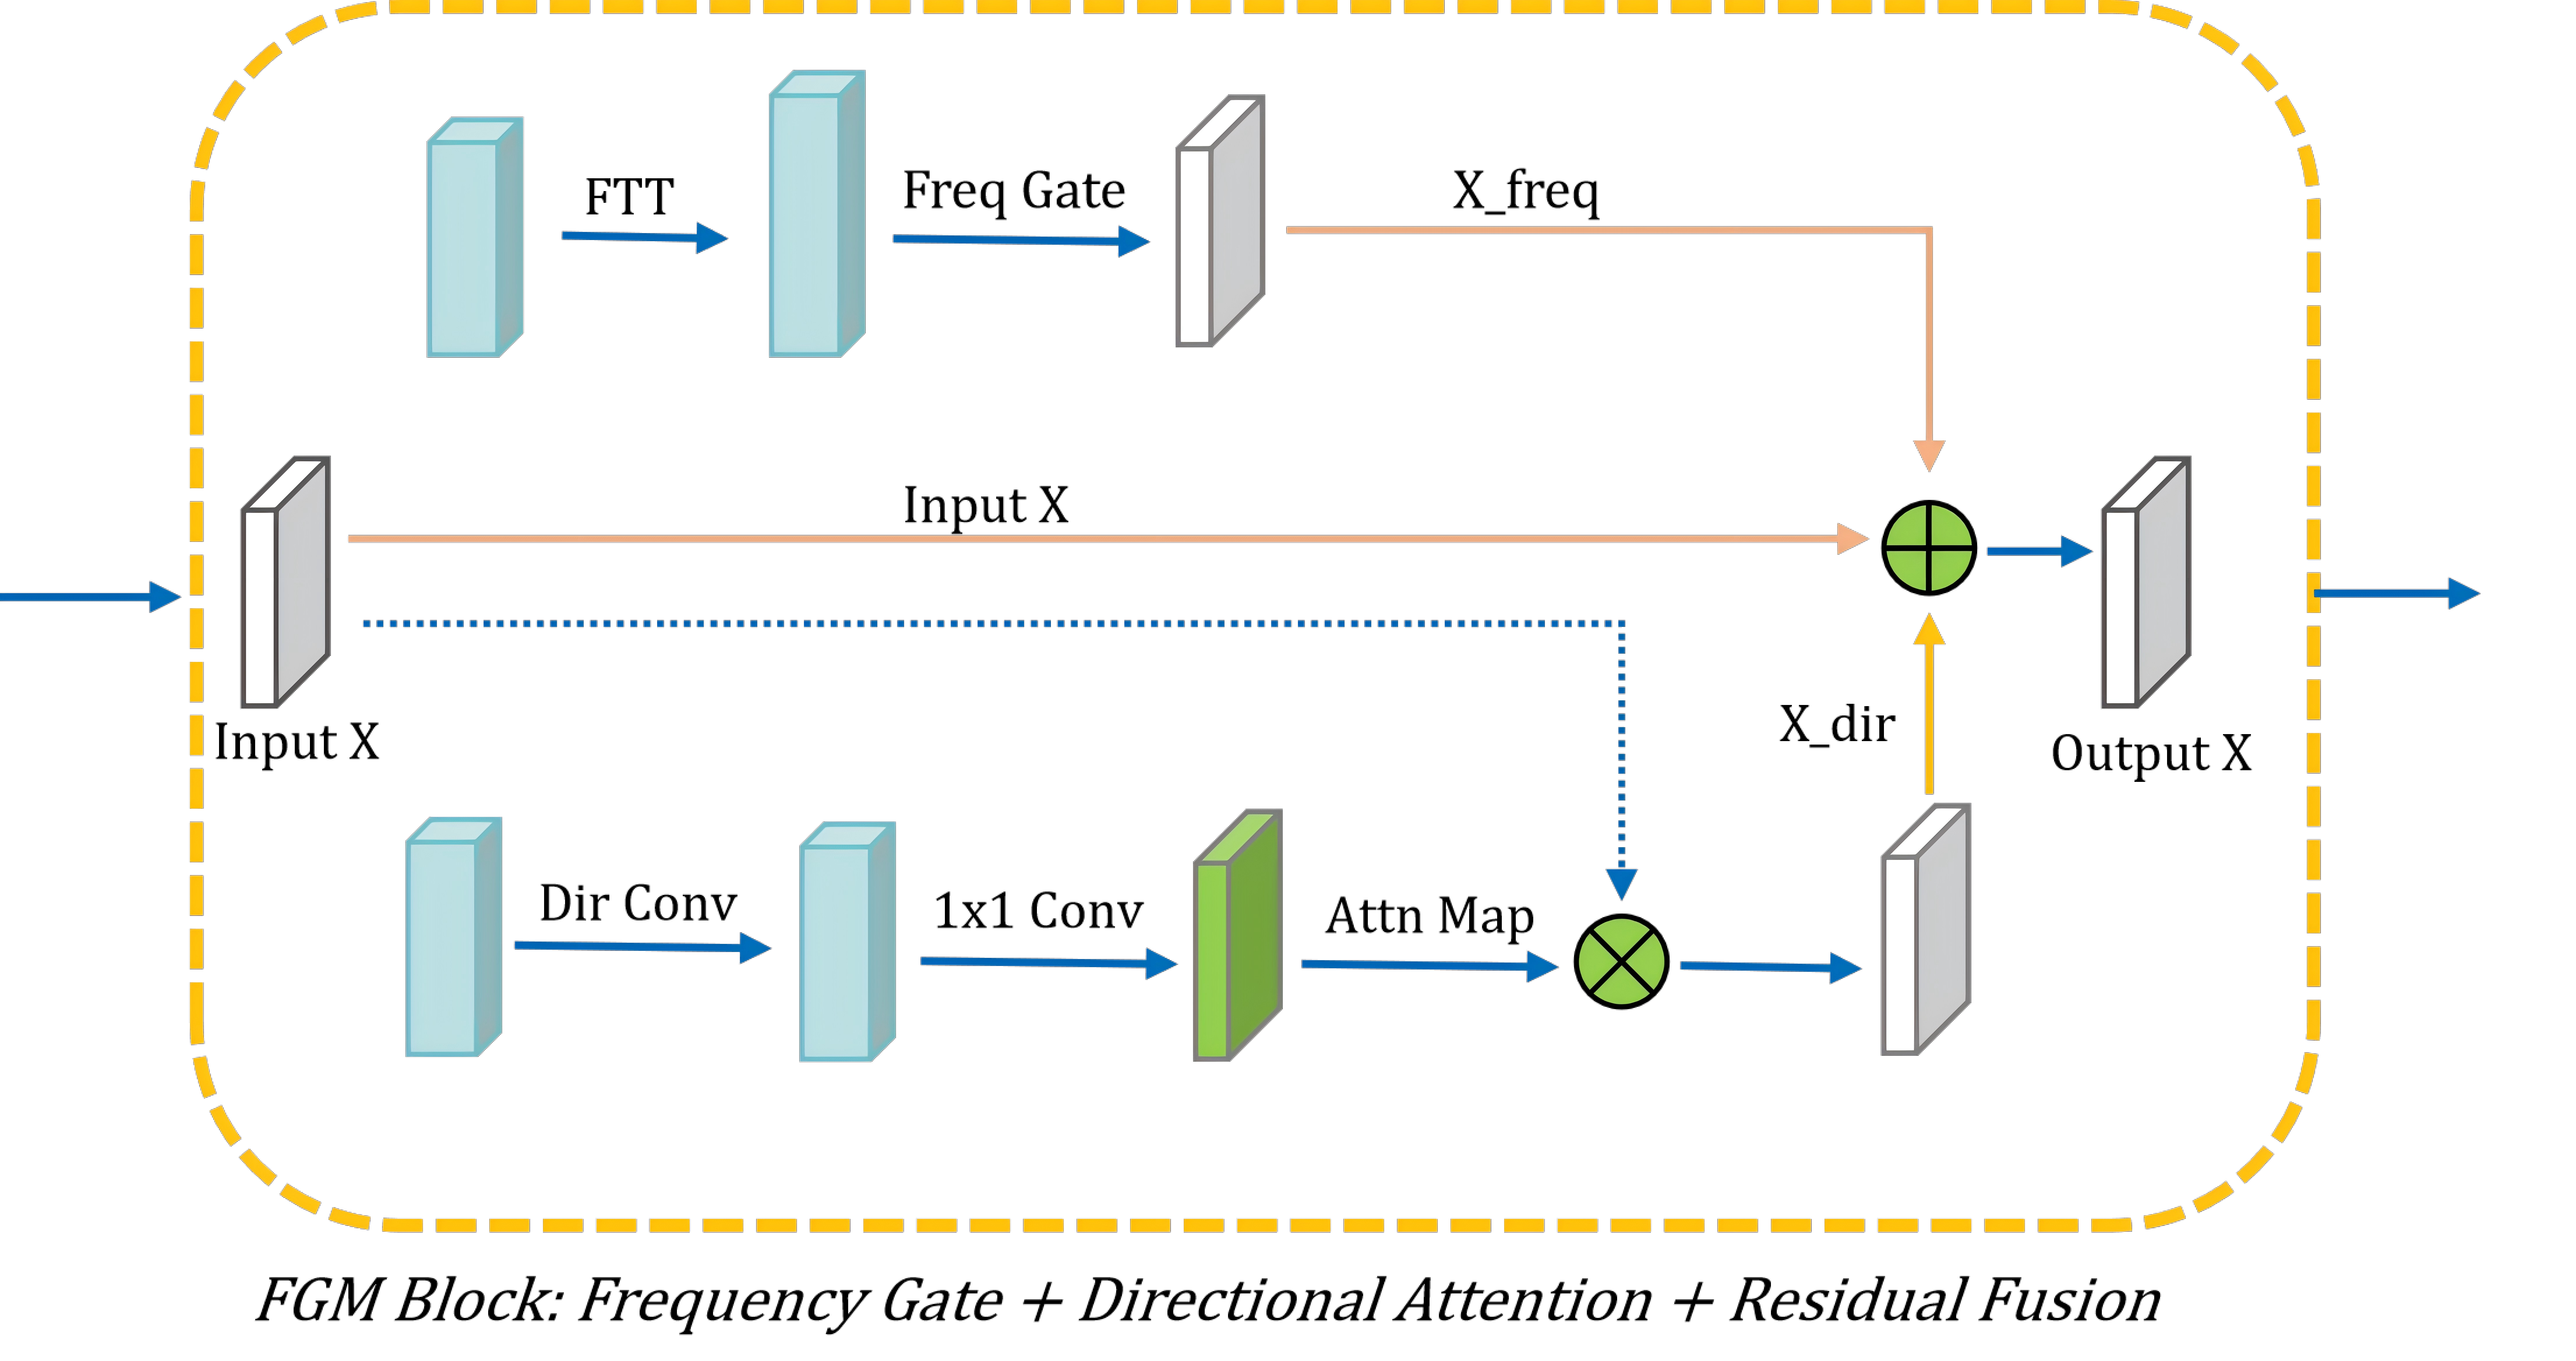
\includegraphics[width=\textwidth]{image/chap04/框架仅模块.png}
	\caption{FGM抗干扰模块结构示意图}
	\label{fig:fgm_arch_placeholder}
\end{figure}

图~\ref{fig:fgm_arch_placeholder} 对模块内部的信息流进行了整体展示。左侧白色斜面特征块表示输入特征张量 $\mathbf{X}$，它既是两条增强分支的共同输入，也是最终融合的基准特征。图中上支路体现了频域门控分支的处理过程：首先通过频域变换（\texttt{FFT}）将输入特征映射到频率空间，以显式分离更易集中在高频区域的雨纹噪声和水膜反光干扰；随后\texttt{Freq Gate}模块对高频区域施加可学习门控，使与车道线无关的高频响应受到抑制，而具有结构意义的边缘信息尽量得以保留。该支路末端的白色特征块记为 $\mathbf{X}_{\text{freq}}$，表示经过频域筛选后的增强结果。

图中下支路体现了方向注意力分支的处理过程。方向卷积（\texttt{Dir Conv}）用于提取不同方向上的局部结构响应，随后通过 $1\times1$ 卷积在通道维度上对多方向信息进行压缩与整合，进一步生成浅绿色细矩形所表示的方向注意力图。随后，注意力图\texttt{Attn Map}与原始输入特征在绿色乘法节点处进行逐元素作用，得到方向分支输出 $\mathbf{X}_{\text{dir}}$。这一设计并不直接重建车道线，而是利用方向先验重新分配输入特征的响应强度，使沿车道线延展方向的有效信息得到突出。

图右侧的绿色加法节点表示残差融合过程。该节点接收三路输入：原始输入特征 $\mathbf{X}$ 的残差直连、频域分支输出 $\mathbf{X}_{\text{freq}}$ 以及方向分支输出 $\mathbf{X}_{\text{dir}}$。其中，残差路径用于维持基线特征分布不被过度扰动，两条增强分支则分别从频率选择性和方向连续性两个角度提供补充信息。最终输出的 $\tilde{\mathbf{X}}$ 不是某一单独分支的结果，而是在原始特征基础上叠加两类增强信息后的融合表征。这种结构既保留了原始特征的稳定性，也使模块能够以较小改动实现对雨天干扰的针对性抑制。

\subsection{模块与CLRNet的融合策略}

该抗干扰模块以即插即用的方式嵌入 CLRNet 的特征提取与精炼阶段之间。考虑到不同层级特征图在语义强度和空间分辨率上差异较大，实际应用时可根据主干网络输出层级选择插入位置，以便在不过度增加开销的前提下优先增强对车道线结构最敏感的中高层特征。

经模块增强后的特征图序列 $\{\tilde{\mathbf{F}}_l\}_{l=1}^L$ 替代原始特征图输入跨层精炼模块，后续检测头与车道线表示方式保持与原始 CLRNet 一致。由此，融合后的整体结构可概括为“主干特征提取 - 抗干扰增强 - 跨层精炼预测”的三级流水线。

由于模块主要由 FFT、深度卷积、$1\times1$ 卷积和残差连接组成，不依赖复杂的多阶段重建网络，因此更适合在保持检测框架简洁性的前提下进行工程部署。这也与本文后续在 Orin 平台上开展模型转换和推理加速的需求保持一致。

\begin{figure}[htbp]
	\centering
	\includegraphics[width=\textwidth]{image/chap04/框架图有模块.png}
	\caption{CLRNet\_FGM 结构示意图（改绘自文献~\cite{zheng2022clrnet}）}
	\label{fig:fgm_clrnet}
\end{figure}

如图~\ref{fig:fgm_clrnet} 所示，本文并未改动 CLRNet 原有的整体检测范式，而是在主干网络输出的多层特征进入后续预测与精炼过程之前，引入 FGM 作为特征增强单元。结合当前配置，模块实际作用于 $L_1$ 与 $L_2$ 两级特征流，即先对这两层特征进行抗干扰增强，再将增强后的特征送入对应的检测头与后续跨层精炼流程；$L_0$ 层保持原始路径，不额外插入增强模块。这样安排的原因在于：一方面，$L_1$ 与 $L_2$ 仍保留较充分的空间结构信息，更适合处理雨天场景下车道线的局部断裂、伪边缘和低对比度问题；另一方面，将模块限制在中高层特征上，也有助于控制额外计算开销，避免对基线网络造成过重扰动。

从整体信息流看，FGM 的定位是特征预增强，而不是对 CLRNet 的车道先验精炼机制进行重写。模块的输入对象是主干特征，输出对象是送往后续检测头和精炼单元的增强特征；图中原有的 refinement 关系以及后续预测流程均保持与基线模型一致。由此，FGM 在整体结构中的作用边界是清晰的：它负责改善雨天条件下特征表达的可分性与连续性，为后续的车道定位与跨层细化提供更稳定的输入，而不改变原模型的任务建模方式。这种融合方式既便于解释性能变化来源，也与本文“在尽量保持基线框架不变的前提下提升雨天鲁棒性”的设计目标保持一致。

\subsection{消融实验设置与结果}

为了验证所提模块的有效性，本文围绕“频域门控是否带来增益”以及“双分支联合后能否保持稳定收益”两个问题组织消融实验。具体而言，将基线 CLRNet、加入 Frequency Gate 的单分支配置以及完整 FGM 模块进行横向比较，以分析频域抑噪机制与双分支融合策略的实际贡献；同时结合训练轮次与损失变化，对模块引入后的收敛稳定性进行观察。

表~\ref{tab:fgm_ablation_placeholder} 给出了根据最新实验整理得到的消融结果。整体来看，三组配置的性能差异保持在合理范围内，说明所提模块没有破坏 CLRNet 原有检测框架的稳定性；其中，加入 Frequency Gate 后 F1 由 $59.56\%$ 提升至 $59.65\%$，完整 FGM 进一步达到 $59.70\%$，同时 Precision 和 Recall 相较基线均有所改善。该结果表明，频域抑噪与方向建模的联合设计能够在保持训练稳定性的前提下，对雨天车道线检测带来持续的正向收益。

\begin{table}[htbp]
	\centering
	\caption{FGM模块消融实验结果}
	\label{tab:fgm_ablation_placeholder}
	\small
	\begin{tabularx}{\textwidth}{@{}YYYYY@{}}
		\toprule
		方法设置 & F1（\%） & Precision（\%） & Recall（\%） & 最优轮次  \\
		\midrule
		CLRNet 基线 & 59.56 & 59.02 & 60.10 & 20 \\
		CLRNet + Frequency Gate & 59.65 & 59.43 & 59.88 & 20 \\
		CLRNet + FGM & 59.70 & 59.48 & 59.93 & 22 \\
		\bottomrule
	\end{tabularx}
\end{table}

表~\ref{tab:fgm_parameter_settings_real} 汇总了已完成验证的模块化实验的关键超参数。现阶段 Frequency Gate 单分支与完整 FGM 在频域门控阈值、方向分支数量和作用层级等设置上保持一致，差异主要体现在是否启用方向分支。因此，当前性能差异主要来源于模块结构本身，而不是由超参数尺度差异造成。

\begin{table}[htbp]
	\centering
	\caption{当前已验证配置的关键参数设置}
	\label{tab:fgm_parameter_settings_real}
	\small
	\begin{tabularx}{\textwidth}{@{}YYYYYYY@{}}
		\toprule
		配置 & 频域门控 & 方向分支 & 阈值 & bins & apply levels & 残差初值 \\
		\midrule
		FG only & True & False & 0.22 & 4 & [1, 2] & 0.08 \\
		FGM one-stage & True & True & 0.22 & 4 & [1, 2] & 0.08 \\
		\bottomrule
	\end{tabularx}
\end{table}


\section{损失函数与训练策略}
\label{sec:loss_training}

\subsection{损失函数设计}

考虑到当前工作重点在于验证抗干扰模块对特征表达的影响，而非重新设计整套检测目标，本文在训练目标上总体保持 CLRNet 原有的监督框架，仅在数据组织与训练流程上针对雨天场景进行适配。

\textbf{车道线位置损失。} 沿用CLRNet的损失定义，对于第$i$条车道线的第$j$个有效行锚点，采用L1损失监督其预测位置与真实位置之间的偏差：
\begin{equation}
	\mathcal{L}_{\text{pos}} = \frac{1}{N_{\text{valid}}} \sum_{i=1}^{M} \sum_{j=1}^{H_r} \mathbb{I}_{ij} \cdot |\hat{x}_{ij} - x_{ij}|
\end{equation}
其中，$M$为最大预测车道线数量，$H_r$为行锚点数，$\mathbb{I}_{ij}$为指示函数，当第$i$条车道线在第$j$行存在时为1，否则为0。$\hat{x}_{ij}$和$x_{ij}$分别为预测和真实的水平位置坐标。

\textbf{存在性分类损失。} 对于每个行锚点，模型还需预测车道线是否存在，采用二值交叉熵损失：
\begin{equation}
	\mathcal{L}_{\text{cls}} = -\frac{1}{M H_r} \sum_{i=1}^{M} \sum_{j=1}^{H_r} [y_{ij} \log \hat{y}_{ij} + (1-y_{ij}) \log (1-\hat{y}_{ij})]
\end{equation}
其中，$\hat{y}_{ij}$为预测的存在概率，$y_{ij} \in \{0,1\}$为真实标签。

\textbf{总损失函数。} 在当前实现中，总损失仍以位置回归损失和存在性分类损失为核心：
\begin{equation}
	\mathcal{L}_{\text{total}} = \mathcal{L}_{\text{pos}} + \alpha \mathcal{L}_{\text{cls}}
\end{equation}
其中，$\alpha$ 为平衡系数。这样的设置有助于将性能变化更直接地归因于抗干扰模块本身，而不是额外的损失项设计。

\subsection{训练策略设计}

针对雨天车道线检测任务的特点，本文采用如下训练策略：

\textbf{两阶段训练。} 第一阶段，在公开数据集 CULane 上进行预训练，使 CLRNet 主干网络和预测头具备基础车道线检测能力；第二阶段，在自建 RainLane 数据集上进行微调，并联合训练抗干扰模块。这样既保留了基线模型对一般车道线结构的先验，也使改进模块能够更集中地学习雨天特有的退化模式。

\textbf{数据采样策略。} RainLane 中包含不同降雨强度和不同光照条件的样本。为避免训练过程过度偏向某一类相对容易的场景，在每个训练轮次中采用分层采样或类别均衡采样策略，使不同降雨强度样本都能被充分看到。

\textbf{学习率与优化器设置。} 训练过程采用适合检测任务微调的优化器与分组学习率策略：对主干网络使用相对较小的学习率，对新引入的 FGM 模块和预测头采用相对更高的学习率，并配合预热与衰减策略提升训练稳定性。这样的安排有利于在保留基线先验的同时，加快抗干扰模块对雨天退化模式的适应。

\textbf{数据增强。} 训练阶段配合第三章已经完成的雨天增强流水线，包括随机水平翻转、亮度与对比度扰动、雨纹合成、水膜反射模拟和局部遮挡增强，以提升模型对真实雨天干扰的适应能力。

\textbf{训练结果组织。} 实验过程中记录损失曲线、验证集指标曲线、最优检查点及关键场景可视化结果。改进模型的最优检查点作为后续模型转换、部署与边缘端推理测试的核心输入。

对于当前已完成端到端部署验证的代表增强配置，其完整训练曲线将在第五章图~\ref{fig:training_curves}中结合部署实验统一给出。整体来看，该配置在前 10 个 epoch 内验证 F1 由 $51.88\%$ 提升至 $58.41\%$，并在第 22 个 epoch 达到最优 $59.82\%$；与此同时，训练总损失由 1.629 下降至约 0.810，其中分类损失降至 0.133，IoU 损失降至 0.381。这说明该配置在保持较快收敛的同时，后期训练过程也较为稳定，并为第五章中的 ONNX 导出与 TensorRT 部署提供了明确的权重选择依据。

\section{本章小结}
\label{sec:summary_4}

本章围绕雨天环境下车道线检测面临的雨滴遮挡、水膜反射和对比度下降等问题，以 CLRNet 为基线模型，给出了抗干扰模块的设计思路与实现说明。通过对基线模型结构的分析，归纳了其在雨天场景下的三类典型失效模式；结合频域特性分析，提出了“频域门控 + 方向注意力”的轻量化改进思路；进一步结合当前代码实现，说明了模块的组成方式及其与 CLRNet 的融合位置，并给出了与之配套的训练目标和训练策略。

本章提出的算法框架为后续实验验证与部署分析提供了方法基础。围绕该模块的整体性能、分支贡献、参数灵敏度及部署适配性，将在第五章中进一步展开分析。

% 注：本章中引用的文献需在论文末尾的参考文献列表中给出完整信息。
% 此处为保持内容连贯，已按开题报告中的文献进行了引用标注。






